\section{Time series and spectrum}

The data series we examine is shown in \autoref{fig:time_series}. The time axis is in bariocentric julian days (BJD) with an offset of 2454833 days (bringing 0 to 1/1/2009). The y-axis is photometric flux, meassured in $\frac{e^-}[s}$. It can be seen that the data undergoes a general drift, increasing in magnitude as time passes.

\begin{figure}[h]
    \centering
    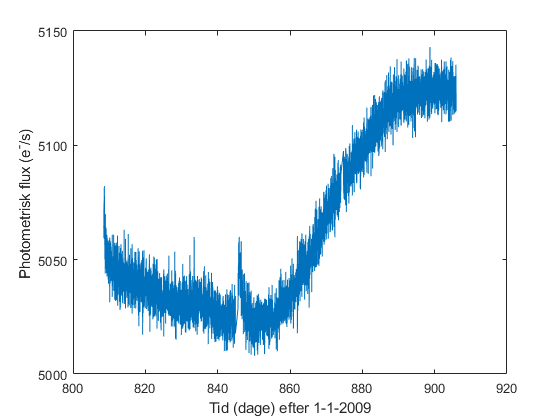
\includegraphics[width = \textwidth]{kep_timeseries.png}
    \caption{Kepler time series}
    \label{fig:time_series}
\end{figure}

The discrete fourier transform (DFT) of the timeseries is displayed in \autoref{fig:smooth_spec}. Note that the frequency is in $\frac{1}{day}$ rather than the usual Hz. This is due to the timeseries being sampled in fractions of days (arround once every half hour (or 0.00056 Hz)).\\
It can be seen in the figure that there is a rather large component with a low frequency. This is probably caused by the general drift in the data.\\ 

\begin{figure}[h]
    \centering
    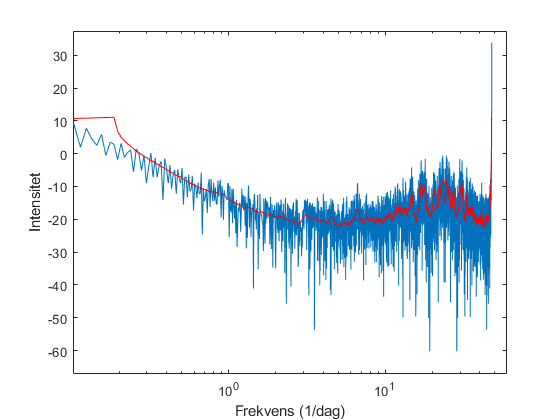
\includegraphics[width = \textwidth]{smooth_spectrum.png}
    \caption{Spectrum of the simeseries and the same spectrum smoothed vit a binsize of 35}
    \label{fig:smooth_spec}
\end{figure}

\autoref{fig:smooth_spec} also shows a smoothed spectrum, with a binsize of 35. It is clear that there is some irregularity in the low frequencies, probably a result of the smoothing including parts beyond the spectrum.\\

The smoothed spectrum removes a large amount of (presumably) noise from the spectrum and highligts a number of peaks. As the timeseries is from a planet survey, it is probable that one or more of these peaks are caused by an eclipse.
